\documentclass{article}

\usepackage{graphicx}
\usepackage[utf8]{inputenc}
\usepackage[T1]{fontenc}
\usepackage[polish]{babel}
\usepackage[linkcolor=blue, colorlinks=true]{hyperref}
\usepackage{titling}
\setlength{\droptitle}{-4em}
\usepackage{enumitem}

\newcommand{\projectname}{UBH}

\begin{document}
	\title{\projectname{} - dokumentacja techniczna projektu (przedmiot: Programowanie Obiektowe, Java)}
	\author{Krzysztof Jajeśnica, nr indeksu 145367, Informatyka, Semestr III}
	\maketitle
	
	\section{Zakres projektu}
		
		\projectname{} jest grą gatunku \href{https://en.wikipedia.org/wiki/Shoot_em_up#Types}{\textit{bullet hell}} w której gracz lata statkiem kosmicznym i niszczy asteroidy oraz statki kosmitów. 
		
	\section{Diagram klas}
		Z powodu dużej ilości klas diagram został podzielony na części. W każdej części kolorem żółtym oznaczono klasy pochodzące z innej części diagramu.
		
		\subsection{Ogólny plan systemu}
			\begin{center}
				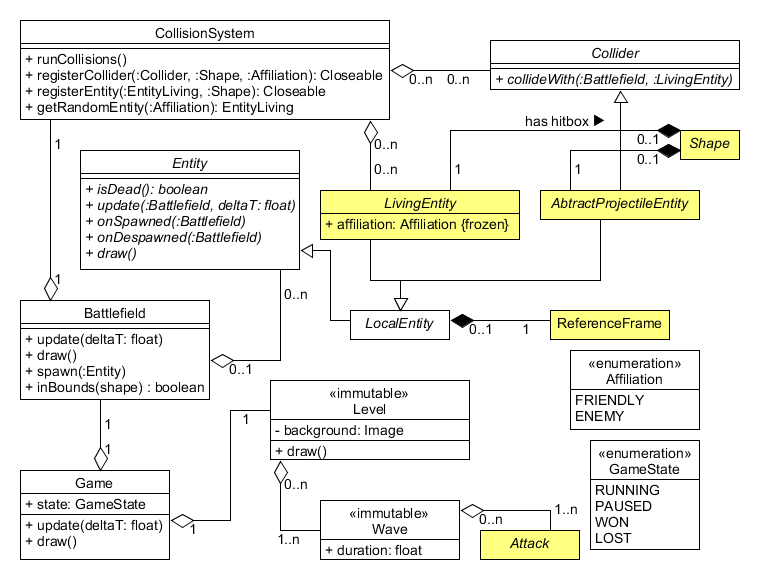
\includegraphics[width=\linewidth]{classdiag-core.png} \\
			\end{center}
		
		\subsection{Klasy pomocnicze}
			\begin{center}
				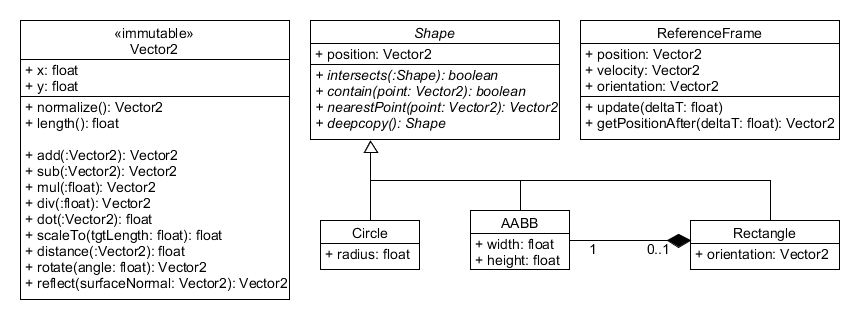
\includegraphics[width=\linewidth]{classdiag-math.png} \\
			\end{center}
	
		\subsection{Ataki}
			\makebox[\textwidth][c]{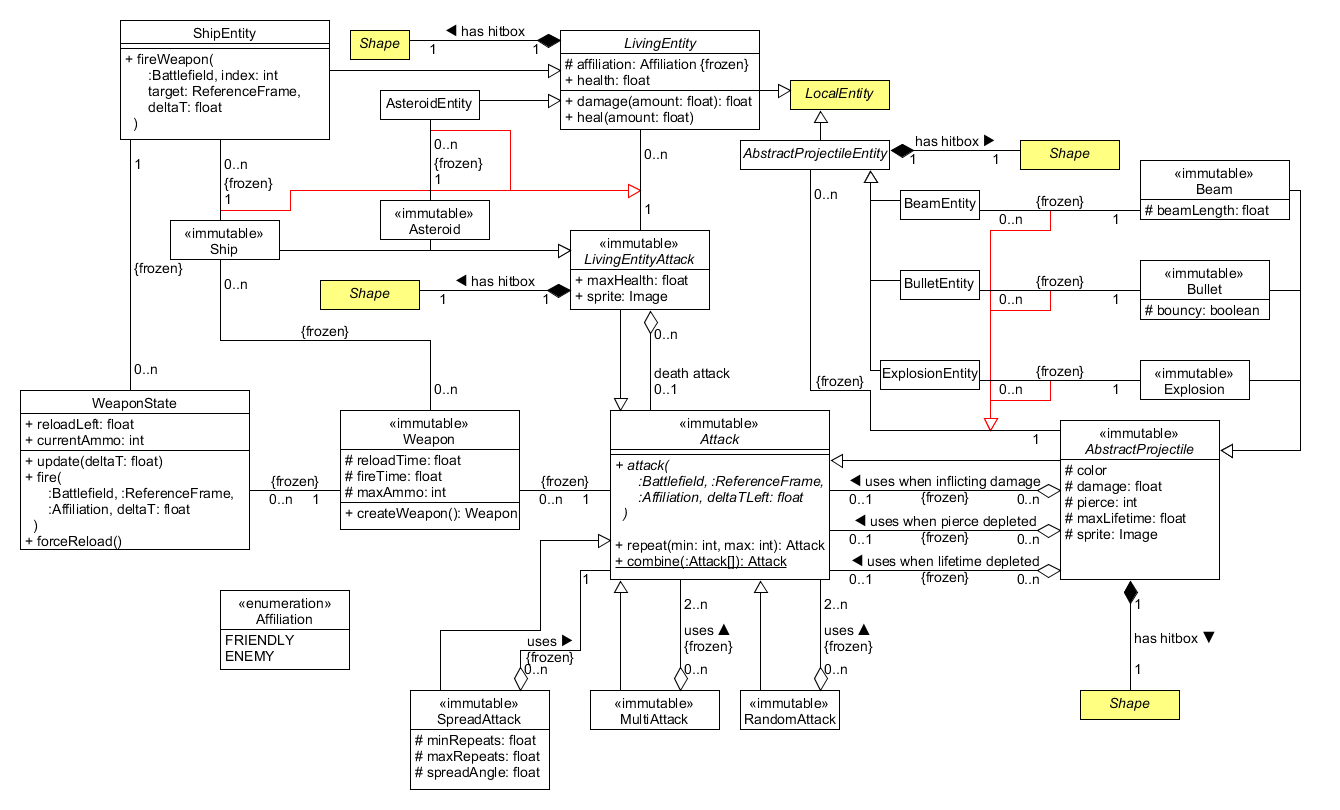
\includegraphics[width=1.6\linewidth]{classdiag-attacks.png}}
			
			Atak (\verb|Attack|) jest abstrakcją opisującą akcję, którą można wykonać by zadać obrażenia bytom żywym (\verb|LivingEntity|) znajdującym się na polu bitwy. Atak zawsze jest wykonywany w pewnym układzie odniesienia (\verb|ReferenceFrame|). Argument \verb|deltaTLeft| jest czasem od użycia ataku do końca obecnej klatki. Wszystkie ataki są immutable, aby umożliwić współdzielenie tego samego ataku przez wiele obiektów.
			
			\subsubsection{Ataki proste}
				Ataki proste bezpośrednio tworzą nowe byty na polu bitwy:
				\begin{itemize}
					\item Podklasy \verb|AbstractProjectile| tworzą pociski.
					\item Podklasy \verb|LivingEntityAttack| tworzą byty żywe (statki, asteroidy, etc.).
				\end{itemize}
			
			\subsubsection{Ataki złożone}
				Ataki złożone składają się z innych ataków i modyfikują sposób ich wykonywania:
				\begin{itemize}
					\item \verb|MultiAttack| łączy wiele ataków w jeden atak.
					\item \verb|RandomAttack| wykonuje losowy atak z listy.
					\item \verb|SpreadAttack| wykonuje dany atak wielokrotnie, przy każdym powtórzeniu modyfikując układ odniesienia, aby rozproszyć efekty ataków na większy obszar.
				\end{itemize}

	
	\section{Wymagania systemowe}
	
		\subsection{Wymagania funkcjonalne}
		
			\begin{itemize}
				\item Gracz może sterować statkiem przy użyciu klawiatury oraz myszki.
				\begin{itemize}
					\item Statek gracza może poruszać się w górę, w dół, w lewo oraz w prawo, ale nie może opuszczać widocznego pola bitwy.
					\item Gracz ma możliwość tymczasowego spowolnienia kontrolowanego statku przez wciśnięcie przycisku.
					\item Gracz może kontrolować bronie znajdującej się na statku. Możliwe jest używanie jednej broni na raz. Gracz może wybierać, którą z broni znajdujących się na statku chce używać.
				\end{itemize}
				
				\item Gra powinna zawierać wiele poziomów.
				\begin{itemize}
					\item Poziom powinien posiadać tło w postaci obrazu.
					\item Poziom powinien zawierać wiele fal przeciwników.
					\item Poziom jest wygrywany w momencie pokonania wszystkich fal przeciwników, a przegrywany w momencie zniszczenia statku gracza.
					\item Gracz ma możliwość powtórnego przejścia danego poziomu dowolną liczbę razy.
				\end{itemize}
				
				\item Gra powinna zawierać różne rodzaje statków gracza.
				\begin{itemize}
					\item Każdy statek jest wyposażony w jedną lub więcej broni strzelających pociskami. Pociski zadają obrażenia kontaktowe.
					\item Każdy statek ma określony rozmiar, wygląd oraz szybkość lotu.
					\item Każdy statek posiada pewną liczbę punktów życia. Wyczerpanie punktów życia skutkuje zniszczeniem statku.
				\end{itemize}
			
				\item Gra powinna zawierać różne rodzaje przeciwników.
				\begin{itemize}
					\item Przeciwnicy mogą być statkami kosmitów lub asteroidami.
					\item Statki kosmitów automatycznie atakują statek gracza przy użyciu broni.
					\item Asteroidy zadają obrażenia przy kontakcie z graczem.
					\item Przeciwnicy mogą używać dodatkowych ataków w chwili zniszczenia (np. eksplodować, stworzyć dodatkowych przeciwników).
					
				\end{itemize}
				
				\item Gra powinna posiadać graficzny interfejs użytkownika.
				\begin{itemize}
					\item Interfejs użytkownika powinien zawierać menu główne, menu ustawień oraz menu wyboru poziomów.
					\item Gra powinna umożliwiać otwarcie menu ustawień podczas gry.
				\end{itemize}
				
				\item Gra powinna umożliwiać tymczasowe wstrzymywanie oraz wznawianie gry.
				\begin{itemize}
					\item Podczas tymczasowego wstrzymania gry gracz ma możliwość przejścia do menu ustawień, zakończenia poziomu lub restartowania poziomu.
					\item Wstrzymywanie gry powinno być kontrolowane przy użyciu klawiatury.
				\end{itemize}
				
				\item Gra powinna umożliwiać definiownie nowej zawartości.
				\begin{itemize}
					\item Gracz może definiować nowe rodzaje statków, asteroid, broni oraz pocisków.
					\item Gracz może definiować nowe poziomy.
					\item Zawartość zdefiniowana przez gracza nie zawiera nowego kodu wykonywalnego.
				\end{itemize}
				
			\end{itemize}
				

		\subsection{Wymagania pozafunkcjonalne}
				
			\subsubsection{Tworzenie nowej zawartości przez gracza}
				Nowe poziomy/bronie/przeciwnicy mogą być definiowane przy użyciu plików w formacie HJSON. Podczas uruchamiania gra parsuje pliki HJSON znajdujące się w ustalonym folderze i tworzy na ich podstawie odpowiednie obiekty. W przypadku napotkania błędnej definicji zawartości gra przerywa ładowanie tej zawartości, informuje użytkownika o wystąpieniu błędu oraz zapisuje dokładne informacje o błędzie do pliku tekstowego. Zawartość zależna od błędnej zawartości nadal zostaje załadowana, ale z pominięciem zawartości błędnej (przykładowo błąd w definicji statku kosmity zapobiega pojawianiu się tego statku we wszystkich poziomach, w których definicji był on użyty). Użytkownik powinien zostać poinformowany o pominięciu błędnej zawartości.
				
				Przykładowy format pliku:\\
				\begin{minipage}{0.5\linewidth}
					\begin{verbatim}
						{
						    type: Asteroid
						    id: small_rock_asteroid
						    maxHealth: 100
						    contactDamage: 50
						}
					\end{verbatim}
				
					Każdy zdefiniowany obiekt ma pewne ID. Definicje obiektów mogą odnosić się do innych obiektów przez ich ID. Zależności cykliczne są zabronione.
				\end{minipage}
				\begin{minipage}{0.5\linewidth}
					\begin{verbatim}
						{
						    type: Asteroid
						    id: medium_rock_asteroid
						    maxHealth: 500
						    contactDamage: 100
						    deathAttack: {
						        type: SpreadAttack
						        minRepeats: 3
						        maxRepeats: 5
						        spreadAngle: 360deg
						        attack: small_rock_asteroid
						    }
						}
					\end{verbatim}
				\end{minipage}

			
			\subsubsection{Praca przy zmiennej liczbie klatek na sekundę}
				
				Gra powinna dostosowywać liczbę klatek na sekundę do możliwości sprzętu użytkownika (zakładamy że z pojedynczą klatką związana jest pojedyncza aktualizacja stanu gry - w diagramie klas metoda \verb|update|). Zmienna liczba klatek na sekundę nie powinna powodować nieprawidłowego działania gry, w szczególności:
				\begin{itemize}
					\item Zmiana liczby klatek na sekundę nie powinna powodować zmiany szybkości działania gry (e.g. jeśli dany pocisk eksploduje po 5 sekundach od pojawienia się na polu bitwy, to powinien to robić z tym samym opóźnieniem niezależnie od tego czy jest 20FPS czy 300FPS).
					\item Częstotliwość strzelania broni powinna być całkowicie niezależna od liczby klatek na sekundę. W szczególności przy strzelaniu z częstotliwością większą od obecnego FPS liczba wystrzelonych pocisków w ciągu sekundy oraz odstępy miedzy pociskami powinny być takie same jak w przypadku FPS większego od częstotliwości strzelania.
				\end{itemize}
			
				Gra powinna działać stabilnie dopóki liczba klatek na sekundę pozostaje powyżej 20FPS.
				
			\subsubsection{Wieloplatformowość}
			
				Gra powinna poprawnie funkcjonować w systemach operacyjnych Windows oraz Linux.
				
			\subsubsection{Łatwość instalacji}
			
				Wszystkie dodatkowe pliki oraz biblioteki konieczne do poprawnego funkcjonowania gry powinny razem z grą znajdować się w pojedynczym pliku .JAR.
			
				
			
	\section{Realizacja projektu}
	
		\subsection{Plan realizacji systemu}
			\begin{center}
				\begin{tabular}{lr}\hline
					Utworzenie działającego prototypu & 2020-12-14 - 2020-12-24 \\
					Implementacja wymagań systemowych & 2020-12-25 - 2021-01-07 \\
					Końcowe testowanie i dopracowywanie projektu & 2021-01-08 - 2021-01-21 \\ \hline
				\end{tabular}
			\end{center}
		\subsection{Wykorzystane biblioteki i narzędzia}
		
			\begin{center}
				\begin{tabular}{ll} \hline
					Biblioteka/narzędzie & Zastosowanie w projekcie \\ \hline
					hjson-java & Parsowanie plików HJSON. \\
					JUnit 5 & Wykonywanie testów jednostkowych. \\
					Gradle & Budowanie projektu. \\ \hline
				\end{tabular}
			\end{center}
		
	\section{Kryteria akceptacyjne}
	
		Razem z wersją 1.0.0 gry na platformie GitHub zostanie umieszczony folder skompresowany \verb|test.zip| zawierający materiały służące do weryfikacji wymagań systemowych:
		\begin{itemize}
			\item Skompilowany program \verb|ubh.jar|
			\item Pliki definiujące dodatkową zawartość: w szczególności \verb|bad_level.hjson| zawierający niepoprawną definicję poziomu, \verb|bad_alien.hjson| zawierający niepoprawną definicję kosmity oraz \verb|good_level_bad_alien.hjson| zawierający poprawną definicję poziomu odnoszącą się do niepoprawnej definicji kosmity.
		\end{itemize}
		Procedura weryfikacji wymagań:
		\begin{enumerate}
			\item Uruchomić \verb|ubh.jar|
				\begin{enumerate}[label*=\arabic*]
					\item Powinien pojawić się komunikat o niepoprawnej zawartości użytkownika.
					\item W folderze powinien pojawić się plik informujący o błędzie w zawartości \verb|bad_level.hjson| oraz \verb|bad_alien.hjson|.
				\end{enumerate}
			\item Przejść do menu wyboru poziomów.
				\begin{enumerate}[label*=\arabic*]
					\item Zweryfikować brak poziomu \verb|bad_level|/informację o błędzie w tym poziomie w liście poziomów użytkownika.
					\item Zweryfikować obecność poziomów \verb|good_level| oraz \verb|good_level_bad_alien| na liście.
				\end{enumerate}
			\item Uruchomić poziom \verb|good_level|.
				\begin{enumerate}[label*=\arabic*]
					\item Powinno wyświetlić się tło poziomu.
					\item Po rozpoczęciu poziomu powinni zacząć pojawiać się przeciwnicy.
					\item Należy zweryfikować możliwość poruszania statkiem, ograniczenie możliwości poruszania do krawędzi pola bitwy, możliwość spowalniania ruchu statku, celowania, strzelania oraz zmiany broni.
					\item Wstrzymać grę.
					\item Zweryfikować możliwość otwarcia menu ustawień oraz powrotu z menu ustawień do rozgrywki.
					\item Wznowić grę.
					\item Zweryfikować otrzymywanie obrażenia od asteroid oraz pocisków przeciwników przez statek gracza.
					\item Pozwolić na zniszczenie statku gracza.
					\item Powinna wyświetlić się informacja o przegranej oraz przycisk służący do restartowania poziomu.
					\item Użyć przycisku do restartowania poziomu. Zweryfikować powrót pola walki do stanu początkowego (ta sama pozycja statku, napełniony pasek punktów życia, brak przeciwników na ekranie).
					\item Zweryfikować możliwość niszczenia kosmitów i asteroid przez pociski gracza. Część kosmitów oraz asteroid powinna wystrzeliwywać dodatkowe pociski po zniszczeniu.
					\item Po pokonaniu wszystkich fal kosmitów powininna się wyświetlić informacja o wygranej z możliwością powrotu do menu wyboru poziomów/menu głównego.
				\end{enumerate}
			\item Uruchomić poziom \verb|good_level_bad_alien|.
				\begin{enumerate}[label*=\arabic*]
					\item Powinien wyświetlić się komunikat informujący o brakującej zawartości.
					\item Poziom nie powinien zawierać żadnych przeciwników (ponieważ był tak spreparowany że jedyny pojawiający się rodzaj przeciwnika to nieprawidłowy \verb|bad_alien|).
					\item Po kilku sekundach powinna pojawić się informacja o wygranej.
				\end{enumerate}
		\end{enumerate}
	
		Ostateczna wersja procedury weryfikacji wymagań systemowych zostanie opublikowana razem z wersją 1.0.0 programu.
		
\end{document}